
% Appendix
%--------------------------------------
\vspace*{45pt}
% Appendix A title (\tituloanexoA) defined in main
\section*{Appendix A - \tituloanexoA}

This appendix documents the main input and configuration screens of the developed web platform. The screenshots show the user workflow from FASTA sequence submission to algorithm, hyperparameter, and step-visualization configuration.

\begin{figure}[!htbp]
\centering
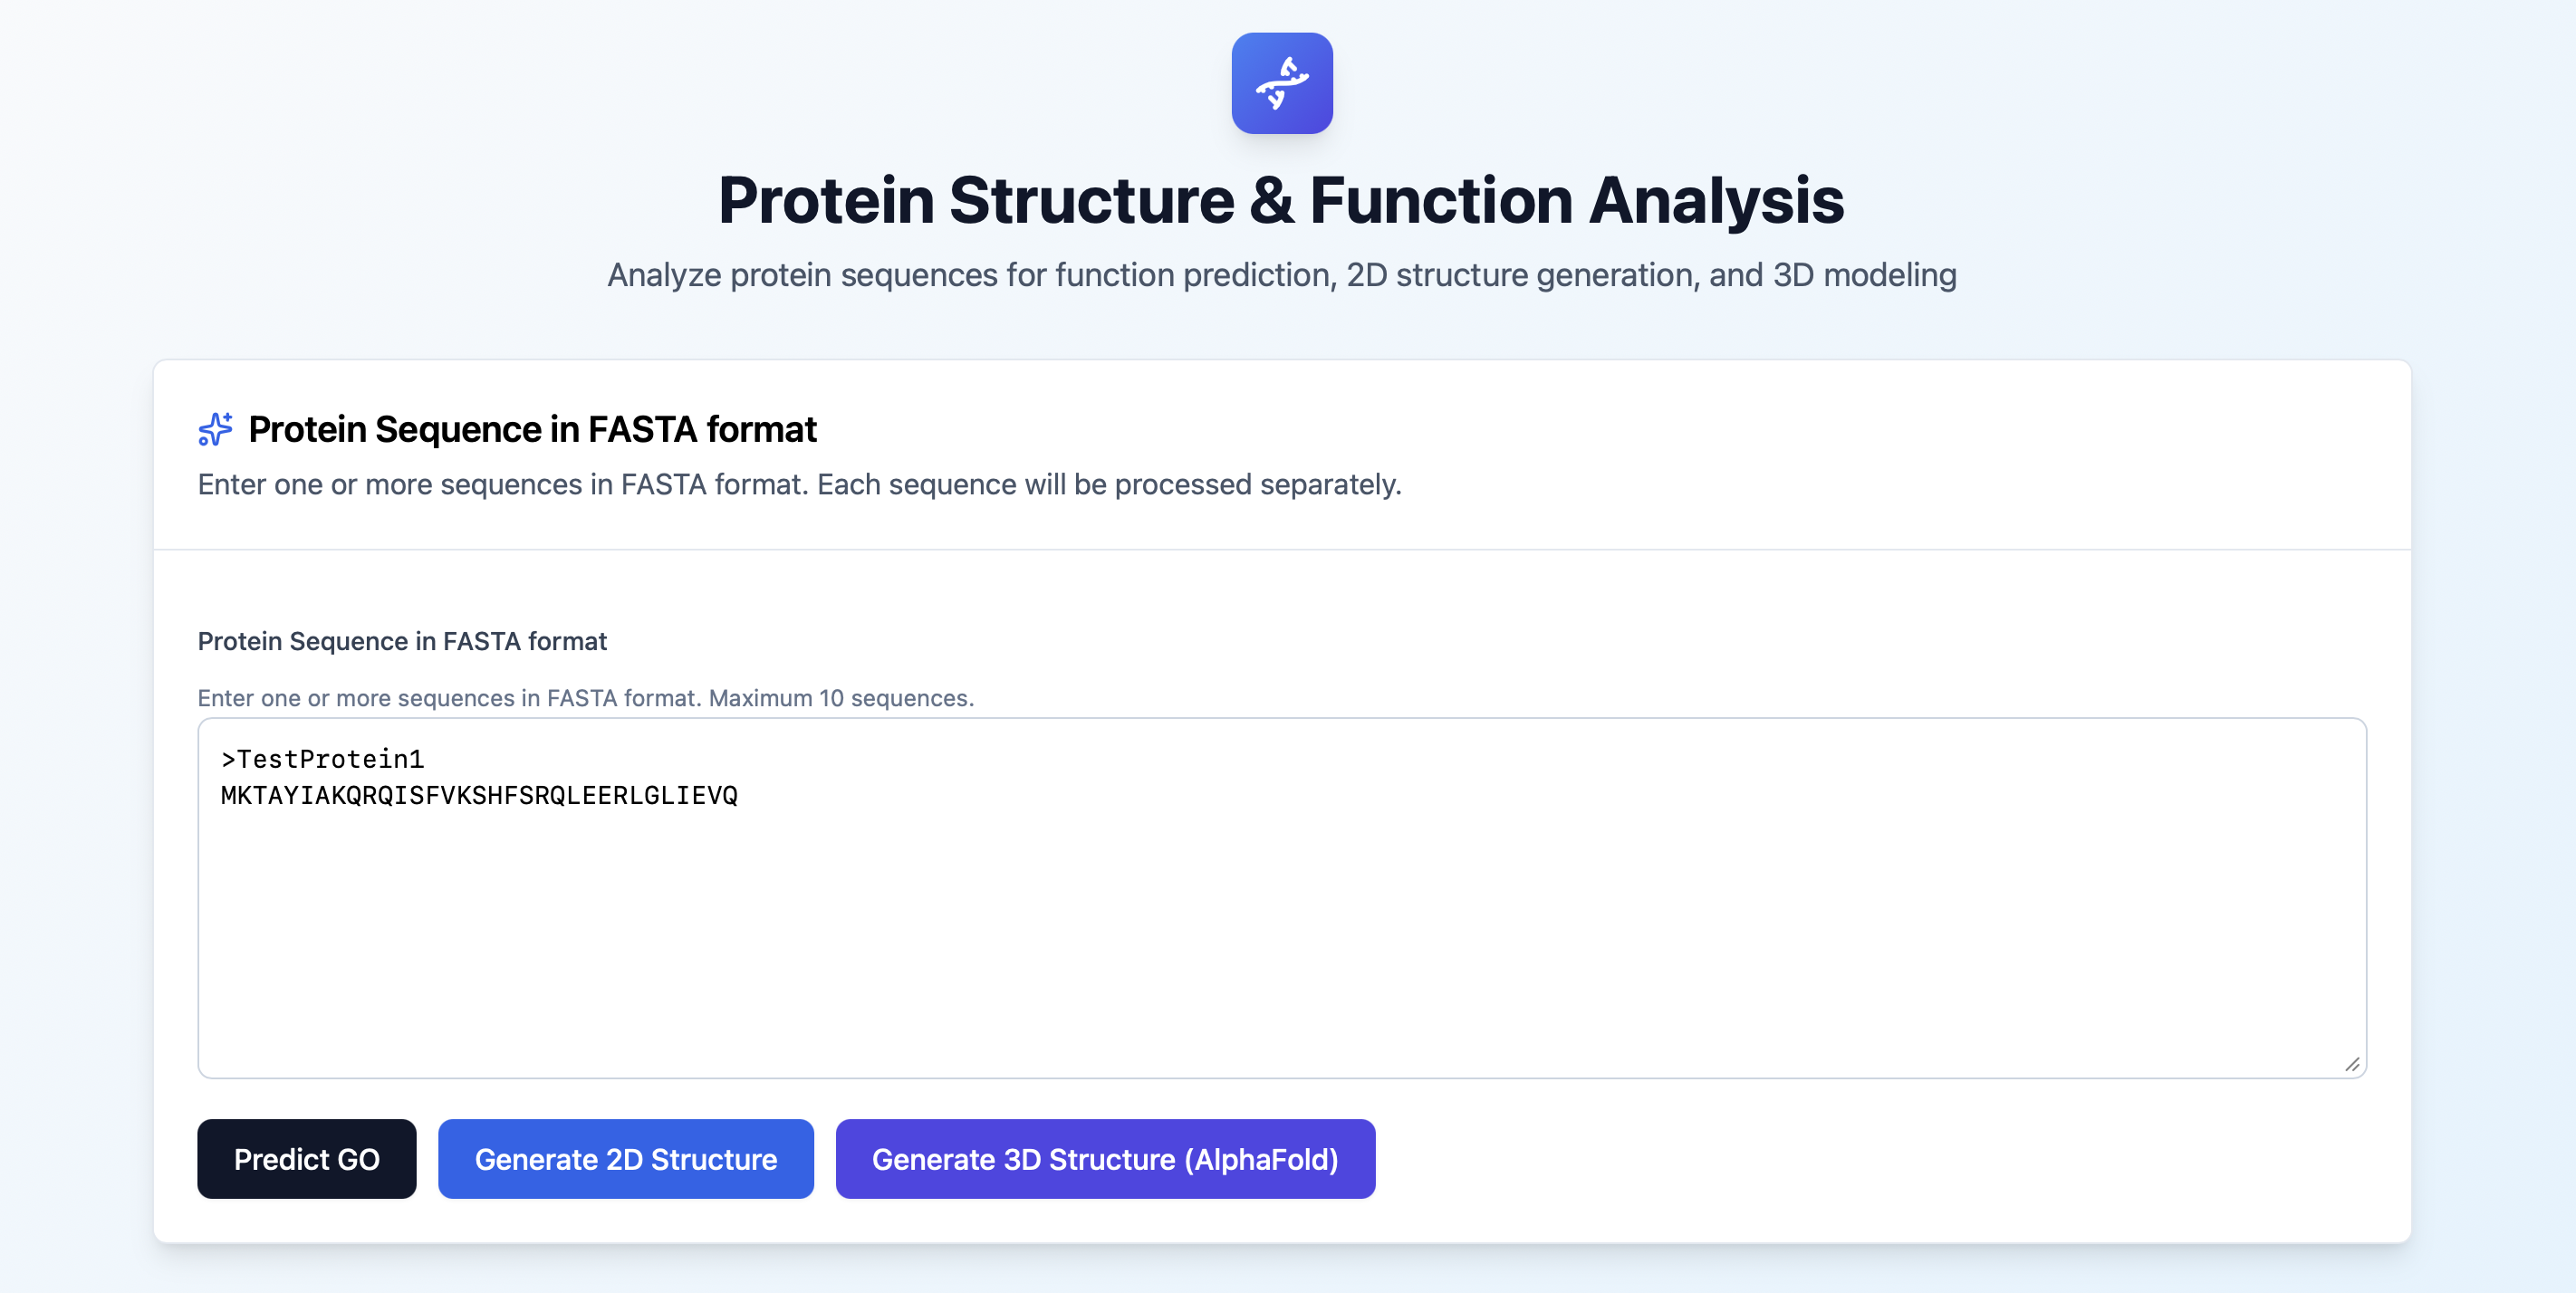
\includegraphics[width=\textwidth,height=0.76\textheight,keepaspectratio]{Figuras/proteinFastaInput.png}
\caption[FASTA input screen]{FASTA input screen of the web platform. Users can submit one or more protein sequences and choose between GO prediction, 2D HP folding, and 3D structure retrieval.}
\label{fig:appendix_fasta_input}
\end{figure}
\FloatBarrier

\begin{figure}[!htbp]
\centering
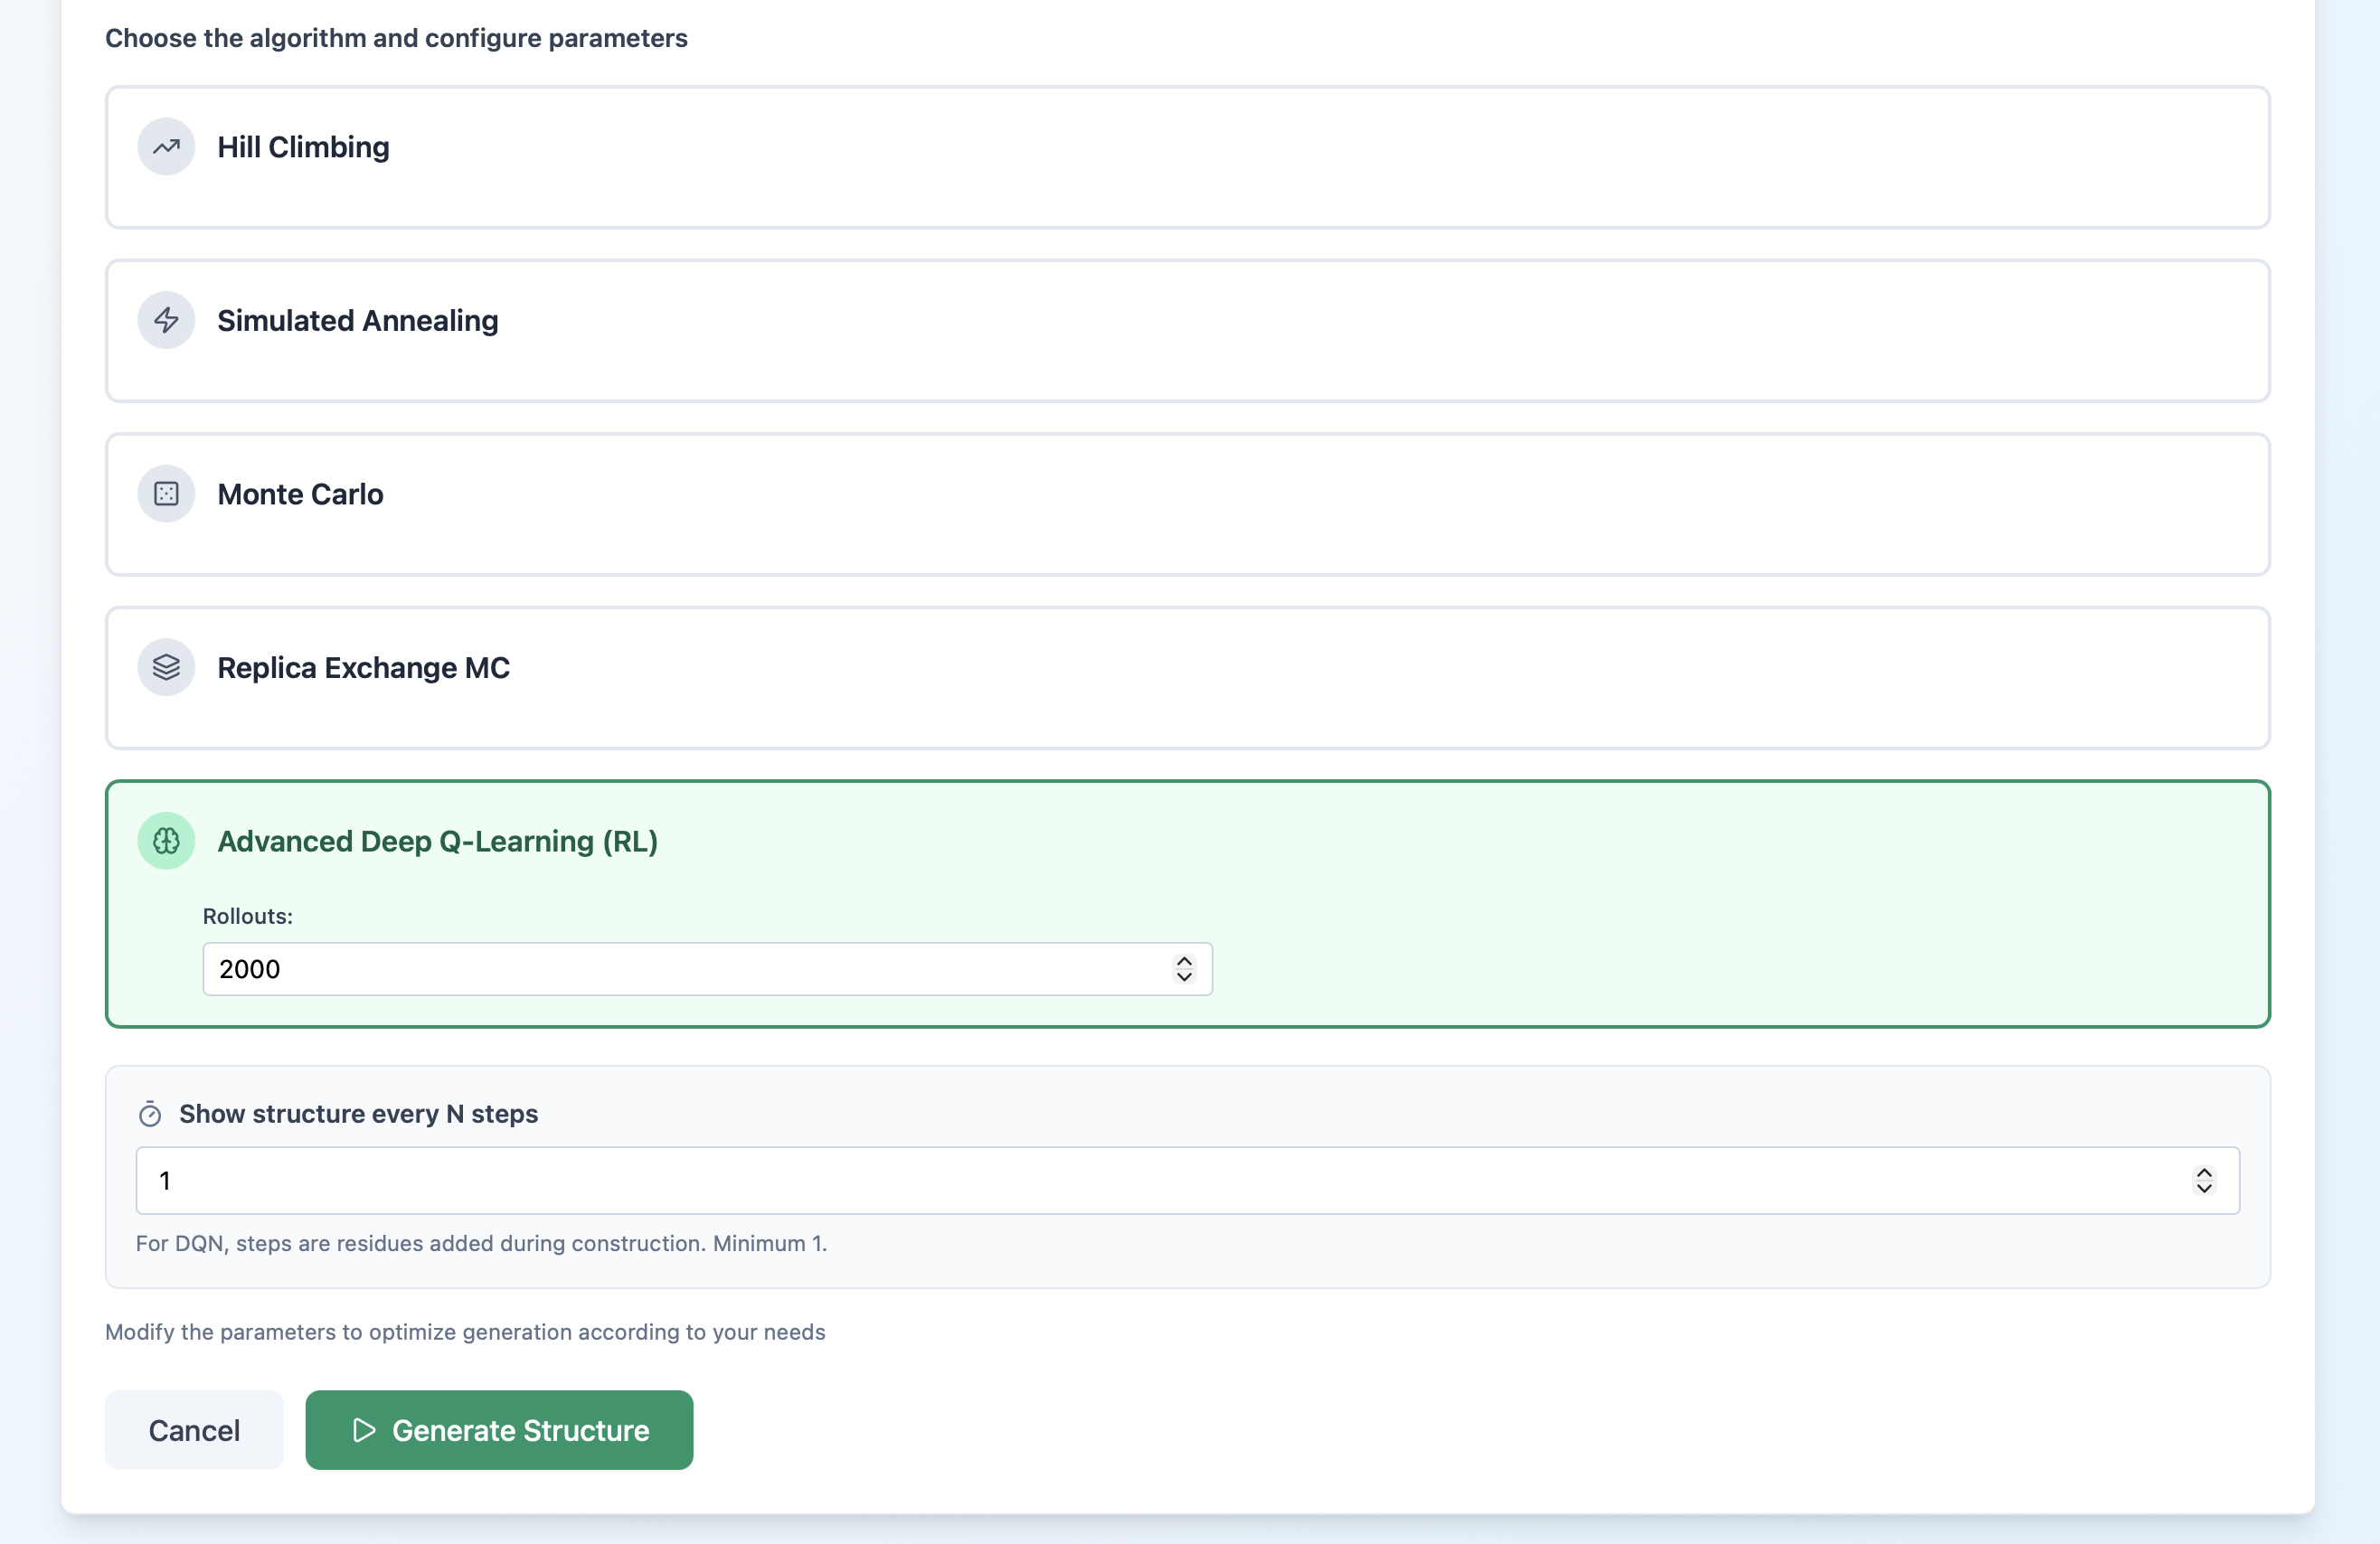
\includegraphics[width=\textwidth,height=0.76\textheight,keepaspectratio]{Figuras/algorithmSelection.png}
\caption[Algorithm selection screen]{Algorithm selection screen for 2D structure generation. The interface exposes the implemented optimization and reinforcement learning methods through a unified workflow. The selected DQN configuration shows the rollout parameter and the step-visualization interval, allowing users to choose how frequently intermediate conformations should be recorded and displayed.}
\label{fig:appendix_algorithm_selection}
\end{figure}
\FloatBarrier

\begin{figure}[!htbp]
\centering
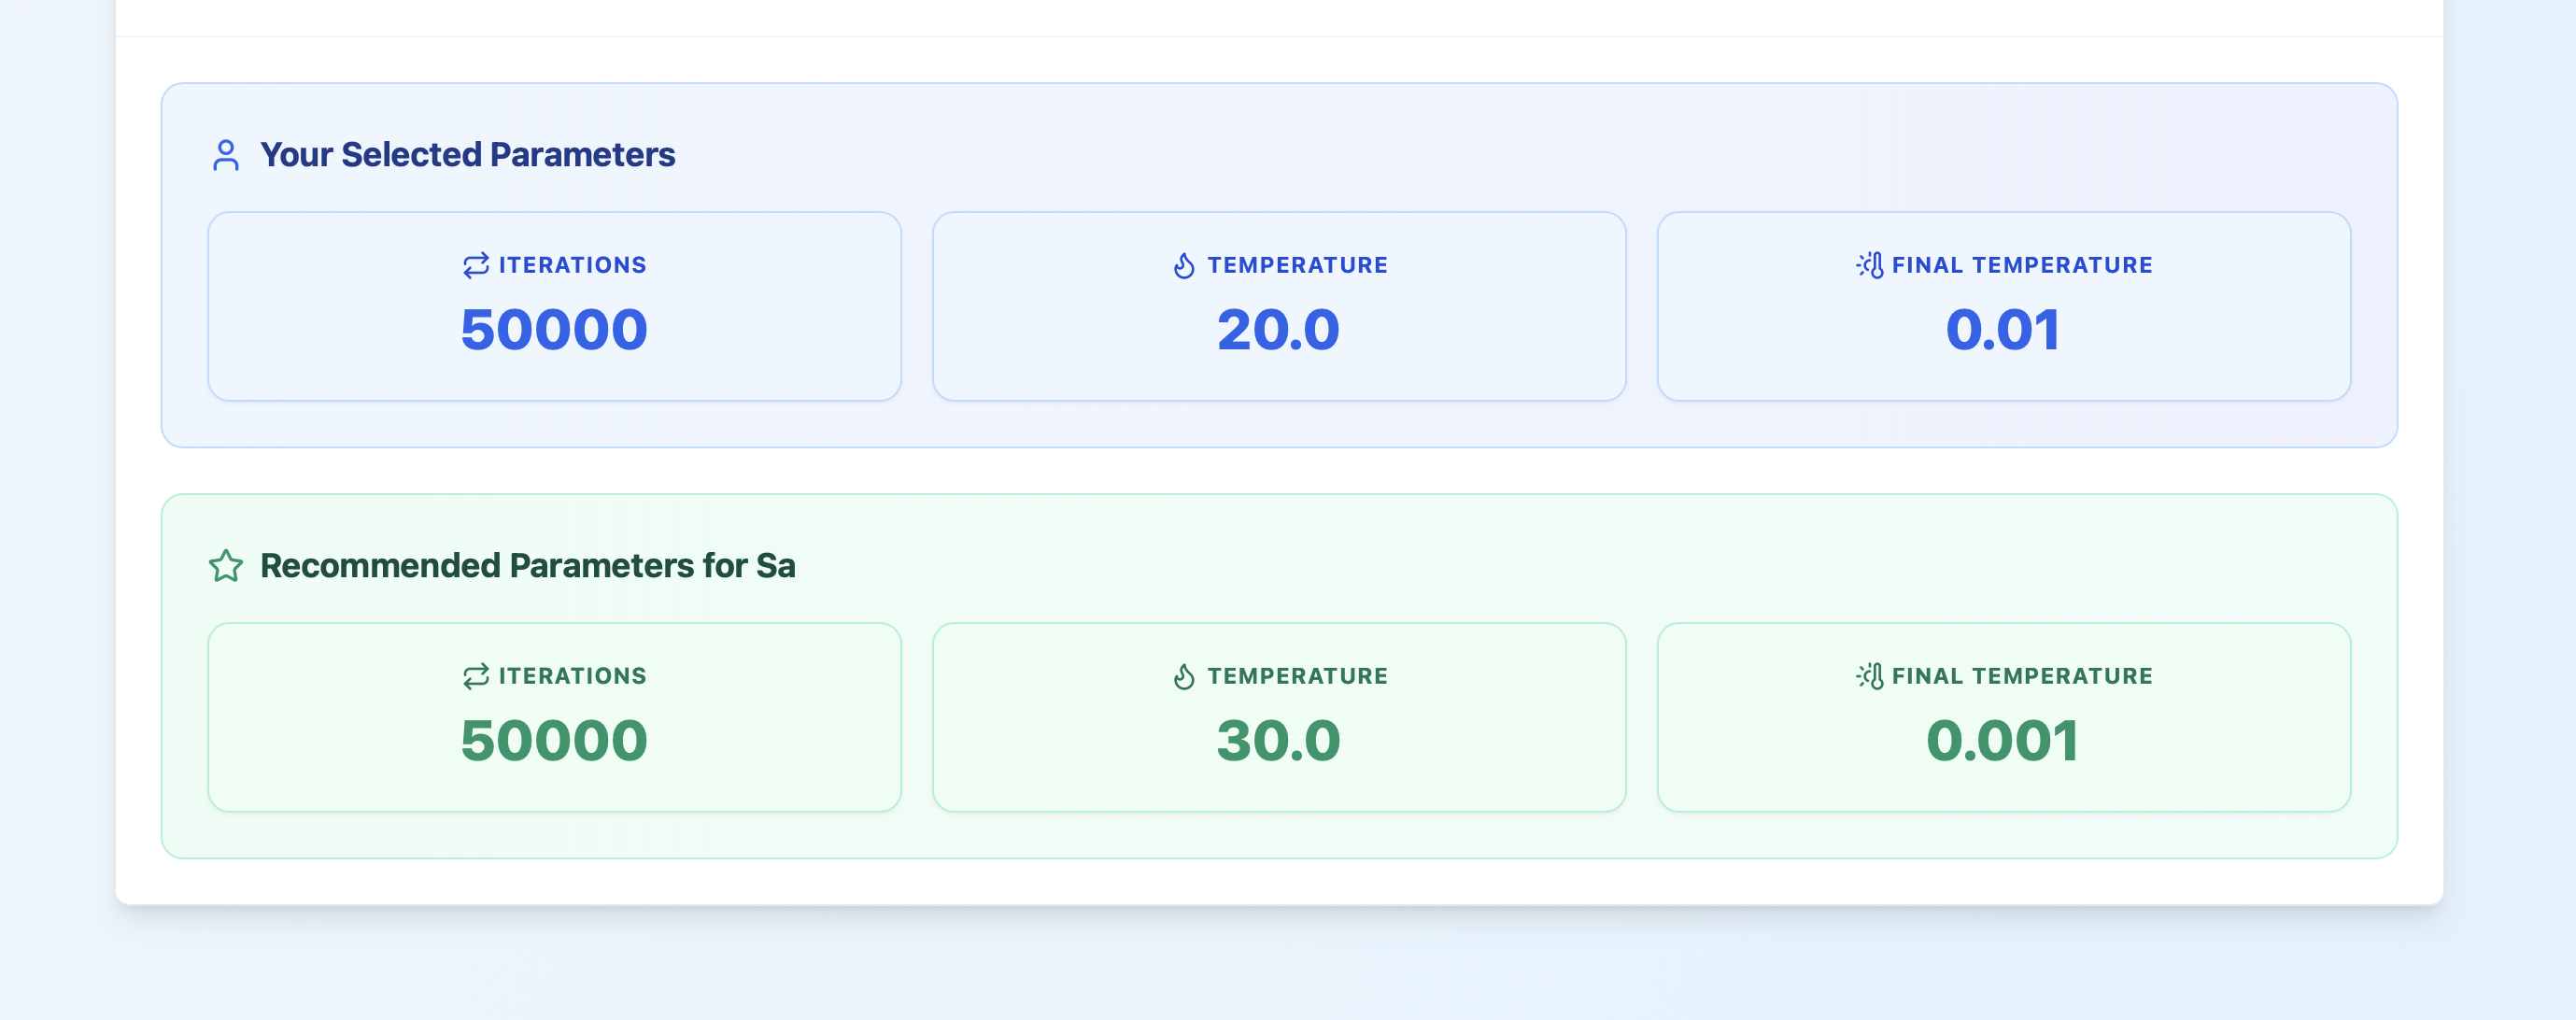
\includegraphics[width=\textwidth,height=0.76\textheight,keepaspectratio]{Figuras/2dStructureParam.png}
\caption[2D structure parameter panel]{Parameter configuration panel for 2D HP structure generation. Algorithm-specific controls allow users to tune iteration budgets, temperatures, replicas, learning parameters, and the interval used by the step explorer to display intermediate folding states.}
\label{fig:appendix_structure_parameters}
\end{figure}
\FloatBarrier
% !TEX root = ../main.tex
